\section{Implementation}
This section will describe the part of the implementation of the Bidirectional Transformations between a RE and a DFA. It will start by describing the reasoning about how to implement the BX and will follow by explaining the implementation process, including some rollback along the way. Finally, it will present the \textit{put} strategy defined for a BX between NDFA and DFA.

The source code of the implementation is available in this Github repository:  \url{https://github.com/lisandrasilva/rv-bx}.

\subsection{Reasoning about BX}
Considering the already existent algorithms to convert between a RE and a DFA, we decided to attempt to implement the BX as a composition of two small BX, more concretely, one between RE and NDFA and another between NDFA and DFA. As depicted in Figure \ref{fig:BX}) the NDFA would be an intermediate structure used as a view in one of the BX and as a source in the another one.  

\begin{figure}
    \centering
    \resizebox{.4\textwidth}{!}{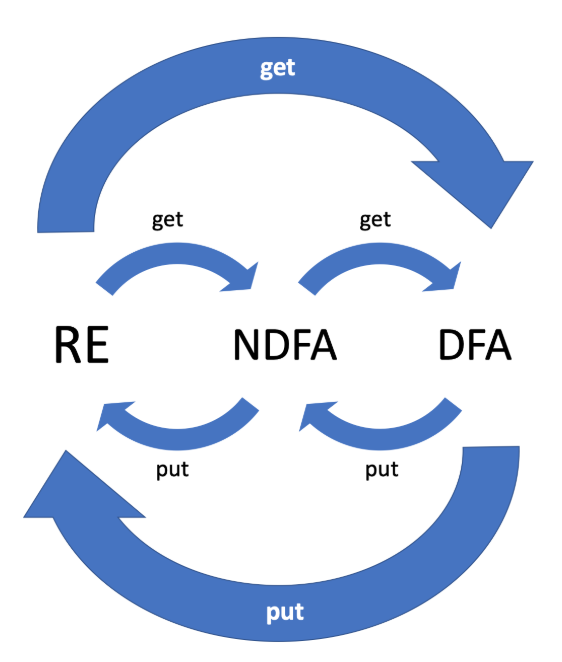
\includegraphics{Images/BX_arc.png}}
    \caption{BX between RE and DFA}
    \label{fig:BX}
\end{figure}

In the BX between RE and NDFA the source is the RE and the view is the NDFA. The \textit{getNDFA} function from RE to NDFA would be one of the conversion algorithms presented on Section \ref{convert} - Thompson's construction or Glushkov's construction. Regarding the BX between NDFA and the DFA, the source is the NDFA and the view is the DFA, where the \textit{getDFA} function would be the Powerset construction algorithm.

\vspace{5mm}
The \textit{get} function that given a RE as source and produces a DFA as view will be the composition of these two functions:

\begin{center}
    \textit{\textbf{get re} = (getDFA . getNDFA) re}
\end{center}

\vspace{5mm}
The main goal is to define the \textit{putback} functions:

\vspace{3mm}
\textbf{\textit{putNDFA}} - function that accepts a NDFA as a source and a possible modified DFA as a view and reflects the changes on the view into the source;
    
\textbf{\textit{putRE}} - function that accepts a RE as a source and a possible modified NDFA as a view and reflects the changes on the view into the source.

\vspace{5mm}
The final \textit{putback} function that accepts a RE as a source and a possible modified DFA as a view and produces the updated RE will be the composition of these two functions:


\begin{center}
    \textit{\textbf{put re dfa} = putRE re (putNDFA (get re) dfa)}
\end{center}

To tackle the problem we decided to start by define the \textit{putNDFA} function.

\subsection{Get function}
As said above the \textit{get} function will be the composition of two, with a NDFA as an intermediate structure. Once this NDFA will be an argument of the \textit{putNDFA} function as the source and \textit{putRE} function as the view, it is necessary to reason about what type of NDFA we should consider, which means reason about the choice for the \textit{getNDFA} function.

The NDFA can be obtained through the Thompson's construction algorithm or through the Glushkov's construction algorithm. But, recall that the resulting NDFA are different since the one obtained through Glushkov's algorithm is \textit{$\epsilon$-free}, while the one obtained through the Thompson's algorithm has $\epsilon$-transitions. 

\subsubsection{NDFA with $\epsilon$-transitions}
Let's consider the NDFA in Figure \ref{fig:epsilon} and its correspondent DFA in Figure \ref{fig:epsilondfa} obtained through the Powerset construction algorithm. 

\begin{figure}
    \centering
    \resizebox{.7\textwidth}{!}{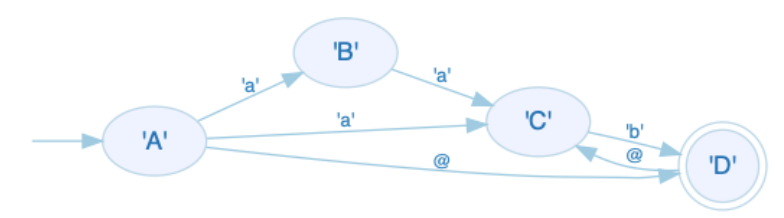
\includegraphics{Images/epsilondfa.png}}
    \caption{NDFA with $\epsilon$-transitions}
    \label{fig:epsilon}
\end{figure}

\begin{figure}
    \centering
    \resizebox{.7\textwidth}{!}{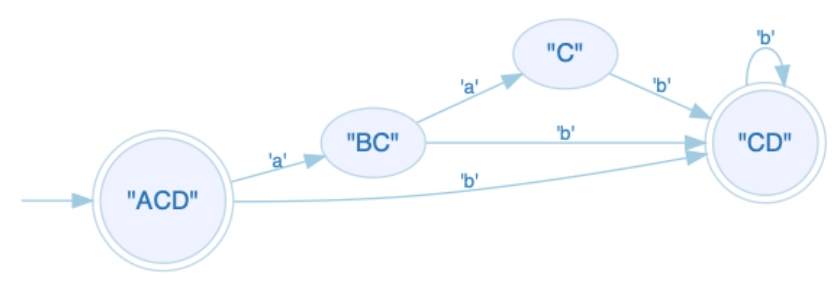
\includegraphics{Images/epsilon_DFA.png}}
    \caption{DFA obtained from NDFA in Figure \ref{fig:epsilon}}
    \label{fig:epsilondfa}
\end{figure}

By analyzing  the pictures the pictures is very hard to reason about a \textit{putback} function when the NDFA has $\epsilon$-transitions. For instance, in the obtained DFA of the given example (Figure \ref{fig:epsilondfa}) all the nodes are dependent on the transitions of the 'C' node in the NDFA, which means that when adding or removing transitions from or to node 'C' in the NDFA, this changes will be reflected in all the nodes with 'C' in the DFA (because that is what is demanded by the Powerset construction).

This fact results in making the possible changes in the view very restrictive, even though we designed a pseudo-algorithm to \textit{put} function in many cases it didn't satisfied the GetPut law. 

\subsubsection{NDFA \textit{$\epsilon$-free}} Figure \ref{fig:glundfa} depicts a NDFA \textit{$\epsilon$-free} equivalent to the NDFA in Figure \ref{fig:epsilondfa}. In Figure \ref{fig:gludfa} is the correspondent DFA. 

\begin{figure}[H]
    \centering
    \resizebox{.8\textwidth}{!}{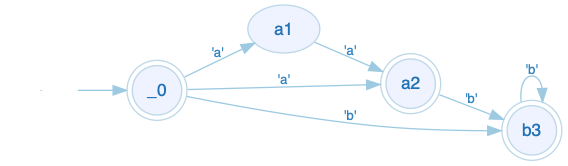
\includegraphics{Images/Glushkovdot.png}}
    \caption{NDFA \textit{$\epsilon$-free}}
    \label{fig:glundfa}
\end{figure}

\begin{figure}
    \centering
    \resizebox{.8\textwidth}{!}{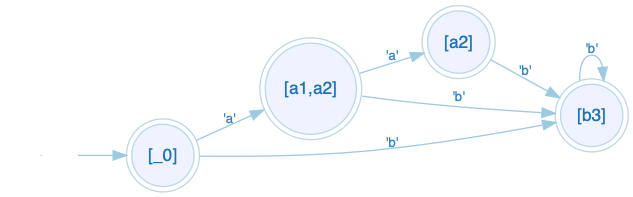
\includegraphics{Images/gluDFAdot.png}}
    \caption{DFA obtained from NDFA in Figure \ref{fig:epsilon}}
    \label{fig:gludfa}
\end{figure}

As we can conclude by analyzing the two automata the dependencies here are less than in the other one, just between nodes \texttt{[a1,a2]} and \texttt{[a2]}, because both have the node \texttt{a2} from the NDFA, and possibly changes in this node will be reflected in both nodes in the view, even only one was modified in the first place. 

However, as it allows a wider range of possible changes on the view we decided to choose the \textit{$\epsilon$-free} NDFA to define the \textit{put} strategy between NDFA and DFA, which means that the \textit{get} function from RE to NDFA should be the Glushkov's construction algorithm. 

\subsection{Put back from DFA to NDFA}

\subsubsection{Structures for DFA and NDFA}
When reasoning about the put back function, the first step was to define the structures to represent both the NDFA and the DFA. Both structures are structurally very similar, but they will differ in the \texttt{delta} function, since in the DFA is not allowed to have two transitions from the same node with the same symbol, while in the NDFA that is possible. 

\begin{verbatim}
data Ndfa st sy = Ndfa { vocabularyN :: [sy ],
                         statesN     :: [st ],
                         initialSN   :: [st ],
                         finalSN     :: [st ],
                         deltaN      ::[((st,sy),st)]
                       }
                   
data Dfa st sy = Dfa { vocabularyD ::[sy],
                       statesD     ::[st],
                       initialSD   :: st,
                       finalSD     ::[st],
                       deltaD      ::[((st,sy),st)]
                     }
\end{verbatim}

We decided to represent the structures with polymorphism on the arguments so they can be more flexible on the types they can represent. However, remind that in the present work, the DFA is result of the Powerset construction of the NDFA, which means that the states in the DFA are sets of the states in the NDFA. As so, for instance, if in NDFA the type of \texttt{st} is \texttt{Int}, then the type of \texttt{st} in the DFA is \texttt{[Int]}.

\subsubsection{Well built DFA}
As the DFA can be edited by the user, and this changes will be reflected in the NDFA, it is important to guarantee that the DFA is well built before proceed with the \textit{put} function. This is guaranteed by the function \texttt{wellBuilt} that ensures the following:

\begin{itemize}
    \item Every transition from a given origin $o$ with a symbol $s$ is unique;
    \item Every Node $x$ must be reachable from the start node;
    \item Every node must reach an accepting node;
    \item For every transition $o \xrightarrow{s} d $, each state in the destination's list of $d$ states must be prefixed by the symbol $s$ (considering the NDFA is result of Glushkov's algorithm and DFA is result of Powerset construction);
    \item The initial state cannot be modified (also a requirement of Glushkov's algorithm)
\end{itemize}

The function returns an error message for each one of the above mentioned rules in case they are violated. 
    
\subsubsection{Reflecting transition table}
The function \texttt{getTable} is responsible for reflecting the DFA transition table into the NDFA transition table. Therefore, it receives as argument the NDFA transition table, the DFA transition table zipped with an accumulator that will save the subset of $d$ of the NDFA transitions that were validated so far, it will also receive the set of states $q$ of the DFA to perform checks and returns the updated NDFA transition table. 

%Each transition \texttt{((o,s),d)} of the DFA is zipped with an accumulator that will save the subset of $d$ of the NDFA transitions that were validated so far. %Thus the DFA table transition received by the \texttt{getTable} function is in fact \texttt{[((([st],sy),[st]),[st])]}. 

\vspace{5mm}
\begin{verbatim}
getTable :: (Ord st, Ord sy) =>[((st,sy),st)] 
                             ->[((([st],sy),[st]),[st)]
                             -> [[st]] 
                             ->[((st,sy),st)]
getTable [] dfaT q = 
    let toAdd = filter (not . null . snd)
                [(((os,d),ds\\rs)) |(((os,d),ds),rs) <- dfaT]
    in concat $ map (`rearrangeS' q)toAdd
    
getTable (t@((o,s),d):ts) dfaT q = 
    let relS = [ x | x <- q , o `elem' x]
        trns = [ 1 | (((os,sym),ds),rs)<- dfaT , 
                                          os `elem' relS ,
                                          sym == s , 
                                          d `elem' ds]
        dfaT' = map (updateListAux t)dfaT
    in if (length relS == length trns) &&(not $ null relS) 
       then t:getTable ts dfaT' q
       else getTable ts dfaT q
\end{verbatim}

\vspace{5mm}
%The function consumes each NDFA transition table recursively. 
For each NDFA transition \texttt{((o,s),d)}, the function verifies that each node in the DFA that contains `$o$' has the transition through symbol `$s$' for a node that contains `$d$'. When this is valid then the NDFA transition is kept in the source and the `$d$' is added to the auxiliary list from the DFA transitions mentioned above (using \texttt{updateListAux} function), otherwise is discarded. 

\begin{verbatim}
updateListAux ((o,s1),d)(((os,s2),ds),rs) = 
            if o `elem' os && s1 == s2 &&d `elem' ds
            then (((os,s2),ds),d:rs)
            else (((os,s2),ds),rs)
\end{verbatim}

When the NDFA transition table is empty it means that all of the old transitions (if existent) were already validated or discarded. At this point, for each DFA transition \texttt{((os,s),ds)} its corresponding auxiliary list with the subset of $ds$ that were already validated is removed from the set $ds$. If the remaining $ds$ list is empty then it means that the transition was already validated. When there are still states in the $ds$ list the new transitions in the NDFA must be created. This is done in the \texttt{rearrangeS} function. 

\begin{verbatim}
rearrangeS :: Eq st => (([st], sy), [st])
                    -> [[st]] 
                    -> [((st, sy), st)]
rearrangeS ((os,sy),dsts) q = 
    let min = [((o,sy),dd) | o <- os \\ (concat $ delete os q), 
                             dd <- dsts]
    in if null min then [((o,sy),dd) | o <- os, dd <- dsts]
       else min 
\end{verbatim}

The function receives a DFA transition, the set of DFA states and creates the list of new NDFA transitions corresponding to the given DFA transition. The \texttt{min} is the list of NDFA transitions in which the NDFA origin nodes that appear in other DFA nodes are removed. 

For instance, taking the example in Figures \ref{fig:glundfa} and \ref{fig:gludfa}, if a new DFA transition is added (([a1,a2],c),[c1]) only the NDFA transition ((a1,c),c1) must be created since if the transition ((a2,c),c1) is also created then when \textit{getting} again the view the DFA would also have the edge (([a2],c),[c1]), that was not created by the user, and so the GetPut law would not be satisfied. When the computed \texttt{min} list is empty it means that is not possible to create new edges without interfere with other DFA nodes, that is called an inconsistency with the source. In this case the function returns all possible NDFA edges for the respective DFA transition, and the inconsistency is dealed with later. 

\subsubsection{Inconsistencies}
Let's take a look at the NDFA and DFA in the Figures \ref{fig:glundfa} and \ref{fig:gludfa} respectively. The NDFA has the transition \texttt{((a2,b),b3)}, which results in the corresponding DFA to have the transitions \texttt{(([a1,a2],b),[b3])} and \texttt{(([a2],b),[b3])}. This strategy allows for instance the user to remove the transition \texttt{(([a2],b),[b3])}, without removing the transition \texttt{(([a1,a2],b),[b3])}, because this transition can exist due to the transition \texttt{((a1,b),b3)} in the NDFA. However, it doesn't allow the user to remove the edge \texttt{(([a1,a2],b),[b3])} without removing the edge \texttt{(([a2],b),[b3])}, since the first is dependent on the second, here we have again an inconsistency with the source, and the second edge is also removed.

When an inconsistency occurs in the view, it means that is not possible to get the same view with the updated source, because the dependencies in the view were not `respected'. In this cases, the user is asked if he wants to proceed with the consistent version of the view, and in that case the source is updated with the consistent version of the view.

\subsubsection{Put Function}
After the table transition of the NDFA is complete it is still necessary to update the other fields of the NDFA structure, this is done by the function \texttt{putNdfaStruct}.

\begin{verbatim}
putNdfaStruct :: (Ord st, Ord sy) => Ndfa st sy  
                                  -> Dfa [st] sy 
                                  -> Ndfa st sy
putNdfaStruct (Ndfa v1 q1 s1 z1 d1) (Dfa v2 q2 s2 z2 d2) = 
        Ndfa v q s z d
    where v = v2
          q = nub $ concat q2
          s = s1
          z = f z1 (concat z2)
          d = getTable d1 (zip d2 (repeat [])) q2
          f [] cz2 = cz2
          f (h:t) cz2 = if h `elem` cz2 
                        then h:(f t (filter (/= h) cz2))
                        else f t cz2
\end{verbatim}

The put of the other fields of the structure is very straight, the most complex is the final states. For that, for each old final state the function tests if it still belongs to some of the new final states and in that case it is kept as a final state or discarded otherwise. In the end the remaining final states are added as final state. 


Finally, the function \texttt{putNDFA} puts it all together: it receives the NDFA, the (possibly) updated DFA and returns an \texttt{Error NDFA}, which is a data type that can contain a NDFA if everything went well or an error message in case the function \texttt{wellBuilt} has returned some error. 

\begin{verbatim}
putNdfa :: Ndfa (Indexed Char) Char 
        -> Dfa [Indexed Char] Char
        -> Error (Ndfa (Indexed Char) Char)
putNdfa ndfa dfa = case wellBuilt dfa of 
                        Ok True -> Ok (putNdfaStruct ndfa dfa)
                        Error m -> Error m
\end{verbatim}

It was also created an interpreter to interact with the user, the interpreter calls the \texttt{putNdfa} function after the user edits the view, and in case the view is not consistent with source asks the user if he wants to continue or to rollback, in case he wants to continue the source and the view are replaced for the consistent versions.